\documentclass[12pt]{article}\usepackage[]{graphicx}\usepackage[]{color}
%% maxwidth is the original width if it is less than linewidth
%% otherwise use linewidth (to make sure the graphics do not exceed the margin)
\makeatletter
\def\maxwidth{ %
  \ifdim\Gin@nat@width>\linewidth
    \linewidth
  \else
    \Gin@nat@width
  \fi
}
\makeatother

\definecolor{fgcolor}{rgb}{0.345, 0.345, 0.345}
\newcommand{\hlnum}[1]{\textcolor[rgb]{0.686,0.059,0.569}{#1}}%
\newcommand{\hlstr}[1]{\textcolor[rgb]{0.192,0.494,0.8}{#1}}%
\newcommand{\hlcom}[1]{\textcolor[rgb]{0.678,0.584,0.686}{\textit{#1}}}%
\newcommand{\hlopt}[1]{\textcolor[rgb]{0,0,0}{#1}}%
\newcommand{\hlstd}[1]{\textcolor[rgb]{0.345,0.345,0.345}{#1}}%
\newcommand{\hlkwa}[1]{\textcolor[rgb]{0.161,0.373,0.58}{\textbf{#1}}}%
\newcommand{\hlkwb}[1]{\textcolor[rgb]{0.69,0.353,0.396}{#1}}%
\newcommand{\hlkwc}[1]{\textcolor[rgb]{0.333,0.667,0.333}{#1}}%
\newcommand{\hlkwd}[1]{\textcolor[rgb]{0.737,0.353,0.396}{\textbf{#1}}}%

\usepackage{framed}
\makeatletter
\newenvironment{kframe}{%
 \def\at@end@of@kframe{}%
 \ifinner\ifhmode%
  \def\at@end@of@kframe{\end{minipage}}%
  \begin{minipage}{\columnwidth}%
 \fi\fi%
 \def\FrameCommand##1{\hskip\@totalleftmargin \hskip-\fboxsep
 \colorbox{shadecolor}{##1}\hskip-\fboxsep
     % There is no \\@totalrightmargin, so:
     \hskip-\linewidth \hskip-\@totalleftmargin \hskip\columnwidth}%
 \MakeFramed {\advance\hsize-\width
   \@totalleftmargin\z@ \linewidth\hsize
   \@setminipage}}%
 {\par\unskip\endMakeFramed%
 \at@end@of@kframe}
\makeatother

\definecolor{shadecolor}{rgb}{.97, .97, .97}
\definecolor{messagecolor}{rgb}{0, 0, 0}
\definecolor{warningcolor}{rgb}{1, 0, 1}
\definecolor{errorcolor}{rgb}{1, 0, 0}
\newenvironment{knitrout}{}{} % an empty environment to be redefined in TeX

\usepackage{alltt}

  %% LaTeX margin settings:
\usepackage{bm}
\usepackage{amsmath}
\usepackage{graphicx, multicol}
\usepackage[margin=.5in]{geometry}
\usepackage{longtable}
\setlength{\parindent}{0pt}
\usepackage{titlesec}
\IfFileExists{upquote.sty}{\usepackage{upquote}}{}
\begin{document}
\large
\begin{center}
{\Large \bf  Homework 2}\\
Claire Rasmussen
\end{center}



\small
\begin{enumerate}
\item Gelman states, "...probabiityies are numerical quantities, defined on a set of 'outcomes,' that are nonnegative, additive over mutually exclusive outcomes, and sum to 1 over al possible mutually exclusive outcomes." We use probability to quantify or characterize the uncertainty surrounding some event. We can make mathematical statements about probability, such as, "The probability of observing a head in one toss of a fair coin is 0.5." Or we can make proability statement that are not mathematical, but largely based on our intuition or general understanding of a system, such as, "There is a good chance that if I go to the store now I'll get stuck in rush hour traffic." 

\item The likelihood principle states that if {\bf x} and {\bf y} are two sample points such that $L(\theta \mid \mathbf{x}) = C(\mathbf{x,y})L(\theta \mid \mathbf{y})$ for all $
\theta$, then conclusions drawn from {\bf x} and {\bf y} about $\theta$ should be the same. The frequentist criticism of the likelihood principle that Jordan made reference to is that this does not allow for infromation about the design of the experiment to enter into the problem. For example, lets say we have a two-sided coin and we're interested in $\theta=P(heads)$. We toss the coin 12 times and let X = the numer of heads. Then $$X \sim Binom(12, \theta)$$ Someone else tosses the coin until 3 tails are observed. Let Y = the number of heads prior to the 2rd tail. Then $$Y \sim NBin(3, \theta)$$ We conduct the two experiments and observe $x=9$ and $y=9$. If we are interested in testing $$H_0: \theta = 0.5 ~vs.~ H_a: \theta > 0.5$$  we draw different conclutions if we let $\alpha=.05$ (we get p-values of 0.075 and 0.0325 in the binomial and negative binomial cases, respectively). By the likelihood prinicple, we should draw the same conclustion about $\theta$, but the frequentists beleive this is flawed logic since the experimental designs differ. Steve gave us this example on 1/28/15 when he first introduced the likelihood principle. One interesting point here is that he presented it as though it were an argument from the likelihoodists as to why the frequentists are wrong. I hadn't thought about from the perspective of the frequentists, that perhaps it isn't valid to expect the same data to yeild the same inference if the conditions under whcih the data were obtained differed. However, regardless of which side one comes at this problem from, I think it really gets at why fixed level testing is a bad idea. In reality 0.075 and 0.0325 really aren't drastically different p-values.

\item 

\item A 

\item In Wilson's example, we are interested in estimating the true duckling survival rate when $100\%$ of our sample ducklings survived. In this case, our MLE would be equal to 1, but we know intuitively the true survival rate is not one. Wilson's point was that when sample sizes are small, it is not uncommon to observe data that results in maximum likelihood estimates on the boundary of the parameter space. Bayesian methods work better here because the use of prior information (even if it is non-informative) has the effect of .

\item ~
\begin{knitrout}\footnotesize
\definecolor{shadecolor}{rgb}{0.969, 0.969, 0.969}\color{fgcolor}

{\centering 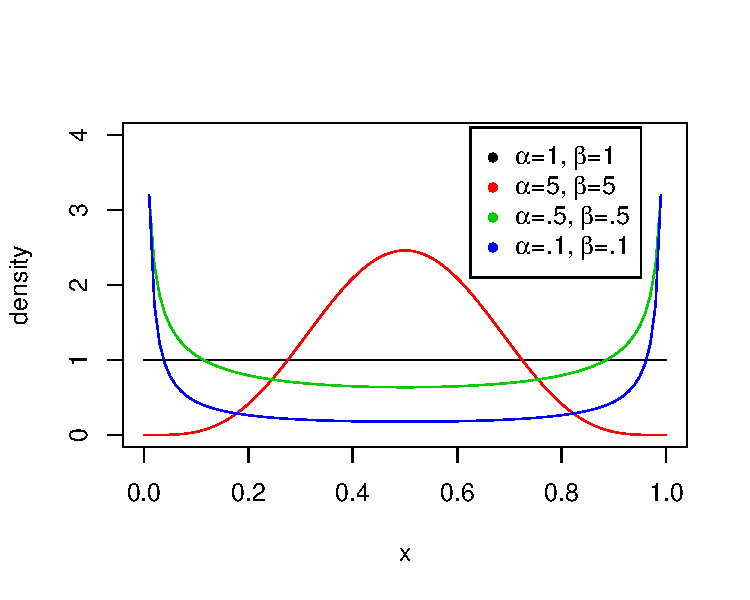
\includegraphics[width=.6\linewidth]{figure/prob6-1} 

}



\end{knitrout}

\item ~
\begin{knitrout}\footnotesize
\definecolor{shadecolor}{rgb}{0.969, 0.969, 0.969}\color{fgcolor}

{\centering 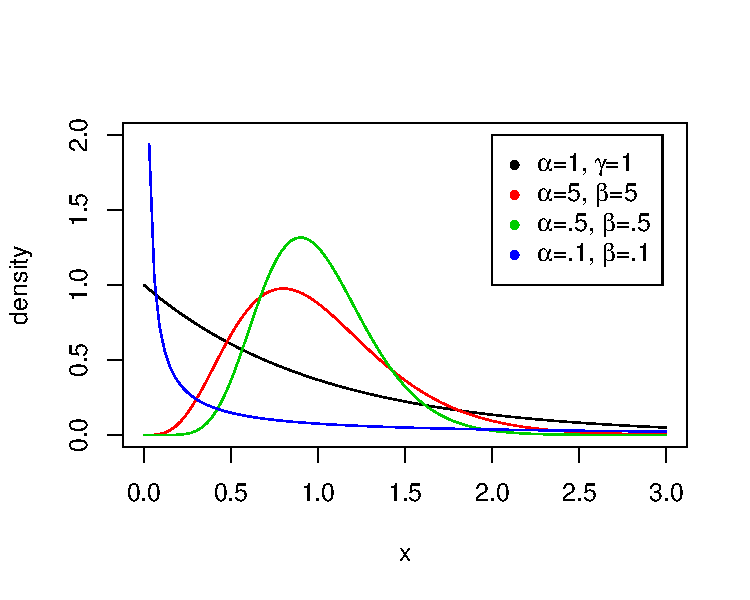
\includegraphics[width=.6\linewidth]{figure/prob7-1} 

}



\end{knitrout}

\item 
\begin{enumerate}
\item$P(Infection \mid + test) = \frac{P(+ test \mid Infection)P(Infection)}{P(+ test)} = \frac{0.92(.05)}{P(+ test \mid Infection) + P(+ test \mid No Infection)} \\
=  \frac{0.92(0.05)}{0.92+.1}= 0.0451$\\
$P(Infection \mid + test) = \frac{P(+ test \mid Infection)P(Infection)}{P(+ test)} = \frac{0.92(.1)}{P(+ test \mid Infection) + P(+ test \mid No Infection)} \\
=  \frac{0.92(0.1)}{0.92+.1}= 0.0902$

\item
\begin{knitrout}\footnotesize
\definecolor{shadecolor}{rgb}{0.969, 0.969, 0.969}\color{fgcolor}\begin{kframe}
\begin{verbatim}
## [1] 0.99
\end{verbatim}
\end{kframe}
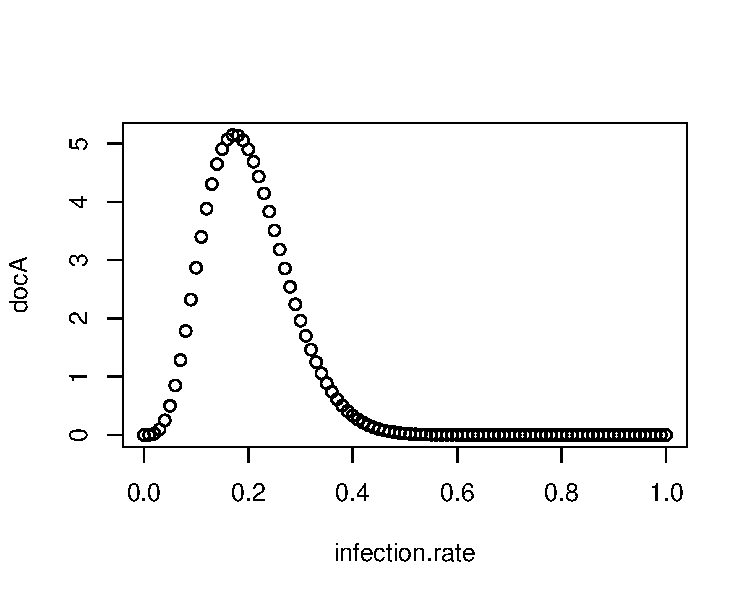
\includegraphics[width=\linewidth]{figure/8b-1} 

\end{knitrout}
\end{enumerate}
\item
\item
\begin{enumerate}
\item 



\item
\item
\item
\item
\item
\item
\end{enumerate}
\item
\begin{enumerate}
\item For $\sigma = 2$, $f(y) = P(\theta=1)f(y \mid \theta=1) + P(\theta=2)f(y \mid \theta=2)$\\

$=0.5*N(1,4)+0.5*N(2,4)$
\begin{knitrout}\footnotesize
\definecolor{shadecolor}{rgb}{0.969, 0.969, 0.969}\color{fgcolor}

{\centering 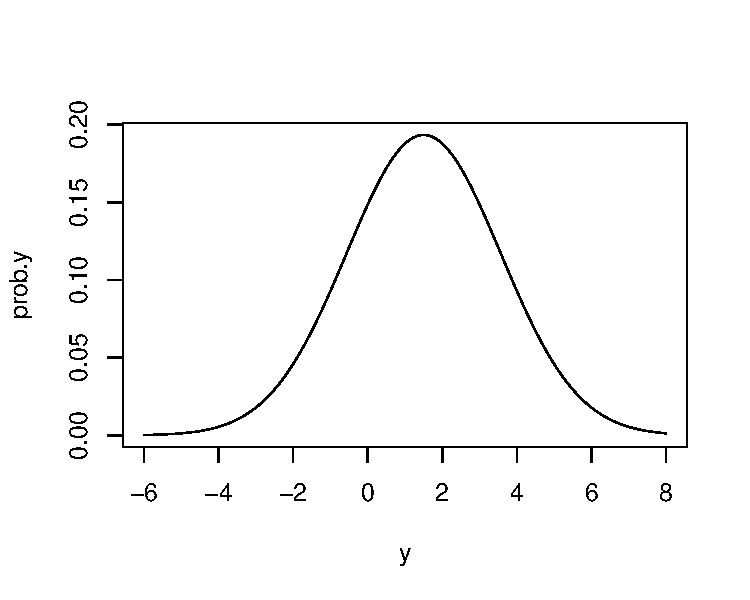
\includegraphics[width=.5\linewidth]{figure/11a-1} 

}



\end{knitrout}
\item Note that $\pi(\theta \mid y)=\frac{f(y \mid \theta)\pi(\theta)}{f(y)}=\frac{f(y \mid \theta=1)P(\theta=1) + f(y \mid \theta=2)P(\theta=2)}{f(y)}$.\\

Then for $\sigma=2$, $P(\theta=1 \mid y=1)=\frac{f(y=1 \mid \theta=1)P(\theta=1)}{f(y=1)}= \frac{0.1995*0.5}{.1878}=0.5312$. Intuitively this makes sense, since our observed datum was closer to $\theta=1$ and $\theta=2$. See appendix for the code used to compute these values.

\item ~

\end{enumerate}
\item $P(Identical)=1/300$, $P(Fraternal)=1/125$\\

$P(Identical \mid Twin Brother) = \frac{P(Identical, Twin Brother)}{P(Twin Brother)}=\frac{P(Twin Brother \mid Identical)* P(Twin Brother)}{P(Twin Brother)}$\\
$=\frac{\frac{1}{300}*\frac{1}{2}}{\frac{1}{2}*\frac{1}{300}+\frac{1}{2}*\frac{1}{125}}=\frac{5}{11}$

\item
\begin{enumerate}
\item Since person A will observe the die roll, he or she will have complete information and will be able to say either the roll result in a 6 or not with probability equal to one. That is, $P_A(E)=1 or P_A(E)=0$. Person B will have only the information that the die is fair, and thus should state that the probabilitiy of observing a 6 is equal to 1/6. That is, $P_B(E)=1/6$.
\item Since person A is ignoran of soccer, he or she has little or no prior information, a logic conclusion is that $P_A(E)=0.5$. Since person B is a knowledgeable sports fan, he or she may have a more informed opionion. Thus, $P_B(E)$ would likely be either less than 0.5 or greater than 0.5.
\end{enumerate}
\item
\item
\begin{enumerate}
\item
\item
\end{enumerate}
\item
\begin{enumerate}
\item
\item
\item
\end{enumerate}
\item
\end{enumerate}

\end{document}
